\section{Data and methodology}
\label{sec:method}

The search looks for one kind of signal: an unresolved carrier at the
star's own position. Such a carrier is narrow compared with a single
correlator channel. Its sky frequency drifts, because the transmitter
accelerates along the line of sight. Over a long track its power is
therefore spread across many channels, and a search that treats each
channel on its own will miss it. The analysis de-drifts the data before
it measures them.

\subsection{The de-drifted search statistic}
\label{sec:statistic}

Each window's dynamic spectrum is stacked along every trial drift rate
$\dot\nu$. The search statistic is the largest stacked signal-to-noise
ratio anywhere on the resulting channel$\times$drift grid,
%
\begin{equation}
T(\mathbf{x})=\max_{\dot\nu,\;\nu}\;
\frac{\sum_{t} I\!\left(\mathbf{x},t,\nu+\dot\nu t\right)\big/\sigma^{2}(t,\nu)}
     {\left[\sum_{t}1\big/\sigma^{2}(t,\nu)\right]^{1/2}},
\label{eq:tstar}
\end{equation}
%
where $I(\mathbf{x},t,\nu)$ is the spectrum at sky position $\mathbf{x}$
in integration $t$ and channel $\nu$, and $\sigma(t,\nu)$ is the noise
scale there. Equation~\ref{eq:tstar} is the matched filter for a
constant-drift carrier. Its numerator adds the signal coherently along
the track and its denominator is the noise of the stacked spectrum, so
$T$ is an absolute signal-to-noise ratio and not a local contrast. The
noise scale is the median absolute deviation across \NCtrl{} control
positions, taken at each integration and each channel. It is therefore
local in time and frequency, global in position, and shared by the star
and every control. The across-position median is never subtracted from
the numerator. The statistic is evaluated at one position at a time,
identically at the star and at each control, which is what makes the two
comparable. $T_\star$ denotes its value at the star.

Spectra are extracted at the star's apparent position, never from images.
For each integration and each native channel the pipeline forms the
weighted vector average of the phase-shifted visibilities, in total
intensity: the mean $I=(XX+YY)/2$ of the two parallel-hand
correlations. That average is the dirty-map value at the
extraction position: an amplitude, not a deconvolved flux density, so in
a field with extended emission it is not a point-source measurement. The data are used as the archive delivered them, through ALMA's own
calibration and quality assurance, with their flagging carried through
and with no regridding and no deconvolution. All delivered channels are searched,
with no edge-channel trimming. A per-integration median along the
\emph{frequency} axis removes the continuum; no median is taken along
time, so a one- or two-channel feature cannot be removed by it. One
subtlety matters for every power quoted below. The delivered channels are
smoothed, so a channel's effective noise bandwidth is not its separation,
and flux density times channel width is not yet a radiated power. A
response correction computed from the correlator's own channel shape
supplies the difference. It is derived, and validated against the
effective resolutions ALMA reports, in Appendix~\ref{app:conventions}.

Two power quantities carry the main text. The trigger level $P_{\rm
trig}$ is the equivalent isotropic radiated power,
$\mathrm{EIRP}=4\pi d^{2}S\,\Delta\nu$ at distance $d$, of a carrier that
makes $T_\star$ reach $T_{\rm trig}=\StageNullTrig$ in one native channel
of width $\Delta\nu$. It is an internal pipeline level, the power at
which the search fires, and it is neither a sensitivity nor a
significance. The sensitivity is $\mathrm{EIRP}_{90}$, the power the
complete automated selection recovers nine times in ten, and it is
measured rather than assumed. \SelNTone{} synthetic carriers of known
amplitude were injected into calibrated visibilities and recovered
through the unmodified pipeline. They span \SelNUnit{} block--window
configurations, both ALMA arrays, four bands and the sample's full range
of channel widths. For Class~A the result is
$\mathrm{EIRP}_{90}=\EirpNinetyMultA\,P_{\rm trig}$. Every limit quoted in
this paper is an $\mathrm{EIRP}_{90}$, given to two significant figures
beside its native channel width; its error budget is
Table~\ref{tab:p90budget}. The absolute flux scale has been checked twice
from outside. Our extractor reproduces an independent reduction of the
same AU~Mic visibilities to \PxJanRatio\,$\pm$\,\PxJanRatioErr{} on a
\PxJanFluxMJy\,mJy point source. It reproduces the published quiescent
flux density of $\epsilon$~Eridani to
\PxEpsRatio\,$\pm$\,\PxEpsRatioErr{} \citep{Burton2022}. The two checks
share neither band nor array.

The drift range searched is bounded by an acceleration, not by a
frequency. Drift rate and line-of-sight acceleration are one quantity in
two sets of units, $a_{\rm los}=c\,\dot\nu/\nu$, so a ceiling expressed
as $\dot\nu/\nu$ is the same physical limit in every band. The default
ceiling is \DriftCeilLo--\DriftCeilHi\,Hz\,s$^{-1}$\,GHz$^{-1}$, that is
$|a_{\rm los}|\le\AccelCeilMed$--$\AccelCeilMax$\,m\,s$^{-2}$. That is
the acceleration of a transmitter orbiting a solar-type star at a few
hundredths of an au. It is the \citet{Mason2025} fiducial with a
threefold margin, widened for a confirmed exoplanet host whenever the
innermost known planet demands more. The margin is not cosmetic: at unit
margin the search would have been blind to two of the windows that
produced a crossing. The grid is uniform in $\dot\nu$, and fine enough
that a carrier midway between two trials loses no more than
\DriftGridFineHalf{} of a native channel over the longest track. Two
limits are worth stating plainly. The rates searched are the apparent ones at the
telescope, so a deliberately chirped carrier is not distinguished from an
accelerating platform. And a transmitter need not be bound to a
known planet at all, so drifts faster than the ceiling are simply
unconstrained (Fig.~\ref{fig:accel}).

\begin{figure}
\centering
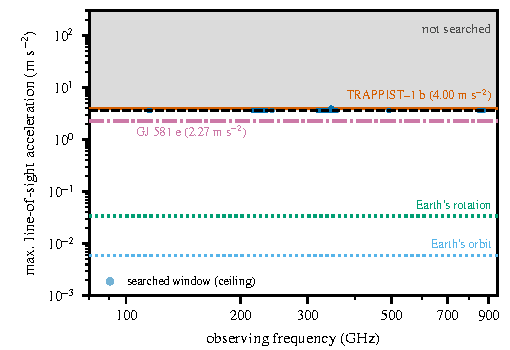
\includegraphics[width=\columnwidth]{figures/drift_acceleration.pdf}
\caption{What the drift search reaches, as a physical selection function.
The drift ceiling of each of the \NWinA{} Class~A windows (points),
converted to line-of-sight acceleration, $|a|=c\,\dot\nu/\nu$, against
observing frequency; the shaded region above is unsearched. The boundary
is flat because the grid was built at constant acceleration; in the units
the search works in it is not, running \AccelDriftLo\,kHz\,s$^{-1}$ at
\AccelFreqLo\,GHz to \AccelDriftHi\,kHz\,s$^{-1}$ at \AccelFreqHi\,GHz.
Horizontal lines are reference accelerations: Earth's rotation
(\AccelEarthRot\,m\,s$^{-2}$ at the equator) and orbit
(\AccelEarthOrb\,m\,s$^{-2}$), and the two most demanding known planets
of any target, \AccelWorstName{} (\AccelWorstVal\,m\,s$^{-2}$) and
\AccelSecondName{} (\AccelSecondVal\,m\,s$^{-2}$). The boundary drawn is
the default ceiling, \AccelCeilMed\,m\,s$^{-2}$, which is also the
median; it runs to \AccelCeilMax\,m\,s$^{-2}$ on the \AccelNWide{}
\AccelWideStar{} windows, and it is each window's own ceiling that
decides whether a given orbit is contained. The most demanding case is
TRAPPIST-1\,b, whose line-of-sight acceleration exceeds the default
ceiling; TRAPPIST-1 transits, so the edge-on figure is the relevant one,
and planet~b lies above the default ceiling for \TrapPhaseHi{} per cent
of its orbital phase and above the widened one for \TrapPhaseLo{} per
cent. It is searchable through the rest of the orbit, and planet~c
reaches the default ceiling only at modest eccentricity.}
\label{fig:accel}
\end{figure}

Only part of the archive can carry a drift search at all, and the two
classes reported here are that division. Channelisation in the sample is
bimodal, with an empty gap between the two modes, so the split is
unambiguous. Class~A is the primary experiment: the \NWinA{} fine-channel
windows, median \ChanAMedKHz\,kHz. In these the maximum searched drift
crosses of order one channel or more over the on-source track, the
condition $\eta_{\rm drift} =
|\dot\nu_{\max}|\tau_{\rm track}/\Delta\nu_{\rm ch} \gtrsim 1$. Class~A
is also the only class with measured end-to-end recovery of a drifting
carrier. Class~B is the secondary experiment: the \NWinB{} coarse-channel
windows, mode \ChanBModeMHz\,MHz, in which a carrier stays inside one
channel for the whole track. These constrain persistent unresolved
spectral excess, carry no drift discrimination, and are never described
as a carrier search here. Each window's own $\eta_{\rm drift}$,
trial-drift count and acceleration ceiling are released catalogue
columns. A reader may therefore reclassify on the physical criterion
rather than the instrumental one. The two criteria do not partition the
survey identically, and we do not claim that they do. Results are given
per class, and combined only where that is statistically appropriate.

\subsection{From a crossing to a candidate}
\label{sec:summary}

Every window goes through the same four tests, in this order. Only three
words describe what comes out of them (Fig.~\ref{fig:chain}).

\begin{enumerate}[label=(\roman*),leftmargin=1.9em,itemsep=2pt,topsep=3pt,parsep=0pt]
\item \emph{Crossing.} A channel$\times$drift cell at the stellar
position reaches $T_\star\geq T_{\rm trig}$. This test generates the
crossings; the other three dispose of them.
\item \emph{Line attribution.} The crossing's frequency is compared with
catalogued molecular transitions in the \emph{star's} frame. Within
$\pm\MaskHalfKms$\,km\,s$^{-1}$ of one of them the crossing is
astrophysical and goes no further. The half-width follows the Keplerian
line-of-sight velocities of gas surviving beyond a few au,
${\lesssim}13$\,km\,s$^{-1}$, with margin for the star's systemic
velocity. The mask
classifies rather than detects: it is applied after the search, so no
threshold moves and no window goes unsearched. Its cost is that the
survey constrains nothing inside the excluded velocity intervals. Of the
\UnionGHz\,GHz of unique sky frequency covered,
${\approx}\SearchedUnionGHz$\,GHz survives the mask
(Appendix~\ref{app:linemask}).
\item \emph{Spatial screen.} The stellar statistic is compared with the
same statistic at \NCtrl{} control positions. They lie in an annulus
placed by each block's own synthesised and primary beams, so that no
control sits on the star. A crossing in which the star exceeds every
control is a \emph{candidate}. Requiring it costs a factor
$\times\ScrCostA$ in sensitivity, from $\ScrTrigOnlyA\,P_{\rm trig}$ at
the trigger alone to $\EirpNinetyMultA\,P_{\rm trig}$ through the screen,
and the completeness quoted below is charged for it. In a window whose
control ring is noise the cost is only $\times\ScrCostNoise$, because
screening against a ring that peaks at $C\sigma$ is equivalent to raising
the $5\sigma$ trigger to $C$; almost the whole effect comes from
\ScrNBright{} windows of \ScrNWinA{} whose rings contain resolved disc
emission at \ScrBrightLo--\ScrBrightHi$\sigma$ (\ScrBrightStars), where no
carrier near the trigger can pass. \emph{The screen therefore measures
compactness rather than authenticity}, which is why it is applied to
prioritise candidates and not to establish them.
\item \emph{Recurrence.} A candidate that repeats at the same tuning in
an independent epoch of the same star is \emph{confirmed}. This is the
survey's only confirmation criterion, and the archive's uneven temporal
sampling is the main reason it is a weak one.
\end{enumerate}

Most crossings are expected by chance, because a fixed threshold is not a
fixed false-alarm rate. The number of independent channel$\times$drift
cells in a window runs from \TuCellsLo{} to $\TuCellsHi$. The same
$5\sigma$ level therefore buys very different protection in a coarse
single-pointing window and in a finely channelised one on a long track.
The expectation is computed window by window, from that window's own cell
count and the exceedance rate measured at its own control positions, then
summed over the windows searched. It predicts \RsevChanceExp{}
unattributed Class~A crossings against \RsevChanceObsAUnattr{} observed,
about two-thirds of the \NHitsA{} Class~A crossings. $T$ is not shown to
follow any standard distribution under the null, which is why $T_{\rm
trig}$ is a trigger level and never a tail probability.
Appendix~\ref{app:falsealarm} gives the conditioning of the expectation
and the control ensemble it is measured on.

\rankstatus{} The evidence for that is out of sample and independent of
the crossings. On \HoWin{} windows the frozen pipeline had never seen,
the stellar rank has median \HoRankMed{} where $0.5$ is expected if the
star and its controls were interchangeable. The displacement survives
clustering by execution block. Its source is geometric: the control annulus samples a
different radial and noise geometry from the star. A parameter-free
correction, tested prospectively against that geometry, does not restore
a validated null and is not adopted (Appendix~\ref{app:radius}). The
screen also loses power exactly where circumstellar gas is brightest,
because a line filling the primary beam drives the star and the annulus
up together rather than cancelling. Throughout this paper $p$ denotes a
genuine significance level, and no probability computed against the
screen's own null is called one.

Three corrections are applied before the statistic is formed. The
extraction field is chosen so that the star lies inside the delivered
primary-beam field, not merely inside the quoted field of view. The
stellar position is propagated to the observation epoch and used as the
apparent position. On-source time is accounted per integration from the
delivered exposure records rather than from the scan intentions.

A visibility-domain check asks whether a candidate's emission is at the
stellar coordinates rather than elsewhere in the field. It is applied to
every crossing and reported beside the chain rather than inside it,
because it cannot discriminate at threshold: a noise peak at the star
also has flux at the star. It is described in \S\ref{sec:vistest}.

Two demonstrations establish that the chain finds what it is meant to
find. Synthetic drifting carriers injected into real visibilities are
recovered through the unmodified pipeline, which is the injection
campaign of \S\ref{sec:statistic} and the measurement behind every
$\mathrm{EIRP}_{90}$ in this paper.
And $\beta$~Pictoris CO, a real astrophysical feature at a known stellar
position, is recovered and localised in two transitions and
\NStageOneBpicEb{} execution blocks. The second is the survey's positive
control, and it is discussed in \S\ref{sec:bpicval}.

%% REQUEST (04_method.tex owner -> integrator)
%% 1. tab:vocab, tab:interpret and tab:maskladder are DELETED from this
%%    file. The first two carried the "screened event / localised event"
%%    vocabulary that the four-step chain replaces; the third was the
%%    two-frame mask ladder. 05_results.tex has since taken the ladder
%%    over and now does %% GENERATED by ledger_v410.py -- do not hand-edit.
\begin{tabular}{@{}lrrr@{}}
\hline
Half-width (km\,s$^{-1}$) & attributed & unattributed & outrank all controls \\
\hline
$\pm13$ & 15 & 41 & 3 \\
$\pm20$ & 16 & 40 & 2 \\
$\pm30$ & 17 & 39 & 2 \\
\textbf{$\pm50$} & \textbf{18} & \textbf{38} & \textbf{2} \\
$\pm100$ & 18 & 38 & 2 \\
\hline
\end{tabular}
 -- the COLLAPSED one-frame
%%    fragment from NUMBERS.md Job 1 S2, which does not exist in this tree
%%    yet, so the full build currently dies with "File tab_maskladder.tex
%%    not found". That is for the numbers owner, not for me, but it is a
%%    hard build break and somebody has to land the fragment.
%% 2. fig:chain is typeset in sections/05_results.tex but is a method
%%    figure and is now cited here first. Please move the float into this
%%    section, or tell me to host it and I will.
%% 3. The visibility-domain check points at \S\ref{sec:vistest} (in
%%    05_results.tex). If that material becomes an appendix, repoint.
%% 4. fig:funnel's caption in 03_sample.tex cites \S\ref{sec:summary} for
%%    "the list"; the survivor-count list has gone and sec:summary is now
%%    the disposition chain. Suggest repointing that clause to
%%    Fig.~\ref{fig:chain}.
%% 5. NUMBERS to supply, so this section can quote them: \EirpNinetyPctLo and
%%    \EirpNinetyPctHi (the one combined interval on the multiplier) for the
%%    EIRP_90 paragraph, and \SelPNinetyCoarse for a Class B sensitivity,
%%    which the document cannot quote at all today. Also a macro for the
%%    Keplerian half-width, still typed as 13 km/s here, and one for the
%%    threefold drift margin.
%% 6. app:notation is no longer cited from this file; every symbol it
%%    defined is now defined at first use here. tab:quantities and
%%    tab:p90budget are likewise no longer cited from the method.
%% 7. Table 10 (tab:algorithm) in App A is now unreferenced: both its
%%    citations were in this file and the four-step chain replaces it,
%%    which is what the triage asked for. The appendix owner should
%%    delete the float.
%% 8. HEADROOM. Measured marginal cost of this section is 2 pp against a
%%    4-pp budget (main-only build: 21 pp with it, 19 pp with it empty).
%%    The triage also asks the method to absorb the amplitude-completeness
%%    FIGURE (old Fig. 11, fig:completeness) so that EIRP_90 is
%%    demonstrated and not merely asserted. I have not created the float,
%%    because the figures owner is merging and renumbering; one
%%    single-column figure fits here with room to spare. Say the word and
%%    I will host it beside the EIRP_90 paragraph. The two flux-scale
%%    ratios above are the triage's transfer of old D.2.
